\documentclass{article}
\usepackage{fancyhdr}
\usepackage{ctex}
\usepackage[a4paper, body={18cm,22cm}]{geometry}
\usepackage{amsmath,amssymb,amstext,wasysym,enumerate,graphicx}
\usepackage{float,abstract,booktabs,indentfirst,amsmath}
\usepackage{multirow}
\usepackage{enumitem}
\usepackage{xcolor}
\usepackage{tabularx}
\usepackage[most]{tcolorbox}
\usepackage{accsupp}
\usepackage[bottom]{footmisc}
\usepackage{subcaption}
\usepackage{logicproof}
% \usepackage[backend=biber,style=numeric]{biblatex}
\usepackage[xetex]{hyperref}
\usepackage{fontspec}
\usepackage{listingsutf8}
\usepackage{xcolor}
\usetikzlibrary{arrows.meta}
\newcommand\emptyaccsupp[1]{\BeginAccSupp{ActualText={}}#1\EndAccSupp{}}
\setlength{\parindent}{2em}
\setmonofont{Consolas}
\setCJKmonofont{黑体}
% \setmainfont{Times New Roman}
\hypersetup{CJKbookmarks=true,colorlinks=true,citecolor=blue,%
            linkcolor=blue,urlcolor=blue,bookmarksnumbered=true,%
            bookmarksopen=true,breaklinks=true}
\lstset{
    % language = C,
    inputencoding=utf8,
    extendedchars=false,
    showstringspaces=false,
    xleftmargin = 3em,xrightmargin = 3em, aboveskip = 1em,
	backgroundcolor = \color{white}, % 背景色
	basicstyle = \small\ttfamily, % 基本样式 + 小号字体
	rulesepcolor= \color{gray}, % 代码块边框颜色
	breaklines = true, % 代码过长则换行
	numbers = left, % 行号在左侧显示
	numberstyle=\emptyaccsupp,
    numbersep = 14pt, 
    keywordstyle=\color{purple}\bfseries, % 关键字颜色
    commentstyle =\color{red!50!green!50!blue!60}, % 注释颜色
    stringstyle = \color{red}, % 字符串颜色
    morekeywords={ASSERT, int64_t, uint32_t},
	% frame = shadowbox, % 用(带影子效果)方框框住代码块
	frame = single, % 用(带影子效果)方框框住代码块
	showspaces = false, % 不显示空格
	columns = fixed, % 字间距固定
  framesep=1em
} 
\lstset{
    sensitive=true,
    moreemph={ASSERT, NULL}, emphstyle=\color{red}\bfseries,
    moreemph=[2]{int64_t, uint32_t, tid_t, uint8_t, int16_t, uint16_t, int32_t, size_t}, emphstyle=[2]\color{purple}\bfseries,
    showspaces = false, % 不显示空格
    }

\raggedbottom

\title{\heiti\textbf{机器学习实践报告}}
\author{第七次实验 \\ 
武泽恺 10225101429
}
\date{2025年12月15日}


\begin{document}
\maketitle

\section{实验目的}
\begin{itemize}
    \item 理解聚类和降维的基本原理；
    \item 掌握 Python 中 K-Means 聚类和 PCA 降维算法的实现方法；
    \item 学会使用可视化手段分析数据的内在结构；
    \item 通过鸢尾花数据集验证聚类和降维算法的有效性。
\end{itemize}

\section{实验环境}
\begin{itemize}
    \item Python 3.11.7
    \item 主要库：
    \begin{itemize}
        \item \texttt{scikit-learn}
        \item \texttt{numpy}
        \item \texttt{matplotlib}
    \end{itemize}
\end{itemize}

\section{实验数据集}
实验采用鸢尾花（Iris）数据集，该数据集包含 150 条样本，每个样本具有 4 个特征，分为 3 个类别，分别对应三种鸢尾花。

\section{K-Means 聚类实验}

\subsection{算法原理}
K-Means 是一种基于距离的无监督学习算法，其目标是将样本划分为 K 个簇，使得簇内样本的平方误差最小。

\subsection{实验步骤}
\begin{enumerate}
    \item 读取 Iris 数据集；
    \item 选取后两个特征作为聚类输入；
    \item 设置聚类簇数 $K=3$，最大迭代次数为 100；
    \item 执行 K-Means 聚类；
    \item 将聚类结果与真实标签进行对齐，计算聚类准确率；
    \item 计算轮廓系数评估聚类效果；
    \item 使用散点图对聚类结果进行可视化。
\end{enumerate}

\begin{lstlisting}[language=Python]
X_kmeans = X[:, 2:4]
scaler = StandardScaler()
X_kmeans = scaler.fit_transform(X_kmeans)
kmeans = KMeans(n_clusters=3, max_iter=100, random_state=42)
y_pred = kmeans.fit_predict(X_kmeans)
\end{lstlisting}

\subsection{实验结果分析}

可以得到如下的结果：

\begin{itemize}
    \item K-Means 聚类准确率约为 0.96。
    \item 轮廓系数为 0.6736179401141785。
\end{itemize}

如图\ref{fig:kmeans_result}所示， K-Means 聚类准确率约为较高水平，说明聚类结果与真实类别具有较好的一致性。轮廓系数为正值，表明聚类结构清晰、合理。

\begin{figure}[H]
\centering
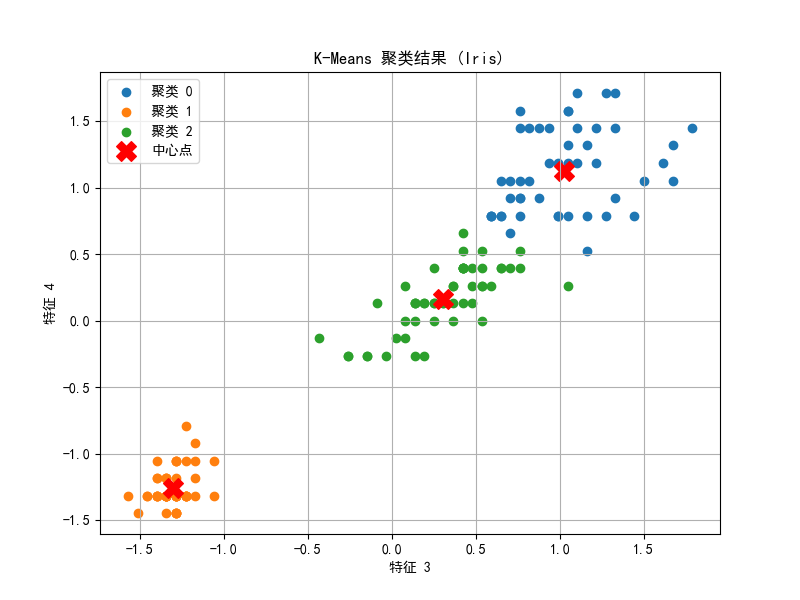
\includegraphics[width=0.8\textwidth]{1.png}
\caption{K-Means 聚类结果 (Iris)}
\label{fig:kmeans_result}
\end{figure}

\section{PCA 降维实验}

\subsection{算法原理}
主成分分析（PCA）通过线性变换将高维数据映射到低维空间，使得投影后的数据方差最大，从而保留主要信息。

\subsection{实验步骤}
\begin{enumerate}
    \item 使用 Iris 数据集的 4 个特征作为输入；
    \item 对数据进行标准化处理；
    \item 分别将数据降至 2 维和 3 维；
    \item 计算各主成分的方差贡献率；
    \item 使用二维和三维散点图进行可视化分析。
\end{enumerate}

\begin{lstlisting}[language=Python]
X_scaled = scaler.fit_transform(X)
pca_2d = PCA(n_components=2)
X_pca_2d = pca_2d.fit_transform(X_scaled)
pca_3d = PCA(n_components=3)
X_pca_3d = pca_3d.fit_transform(X_scaled)
\end{lstlisting}

\subsection{实验结果分析}

我们可以得到如下的结果：
\begin{itemize}
    \item 2 维 PCA 的方差贡献率为 [0.72770452 0.23030523]，累计方差贡献率为 0.9580097536148194。
    \item 3 维 PCA 的方差贡献率为 [0.72770452 0.23030523 0.03683832]，累计方差贡献率为 0.9948480731910934。
\end{itemize}

如图\ref{fig:pca_2d}和图\ref{fig:pca_3d}所示，二维 PCA 已能够保留大部分数据的方差信息，不同类别在低维空间中具有较好的分离性。三维 PCA 进一步提高了信息保留程度，数据分布更加清晰，验证了 PCA 在降维和特征提取中的有效性。

\begin{figure}[H]
\centering
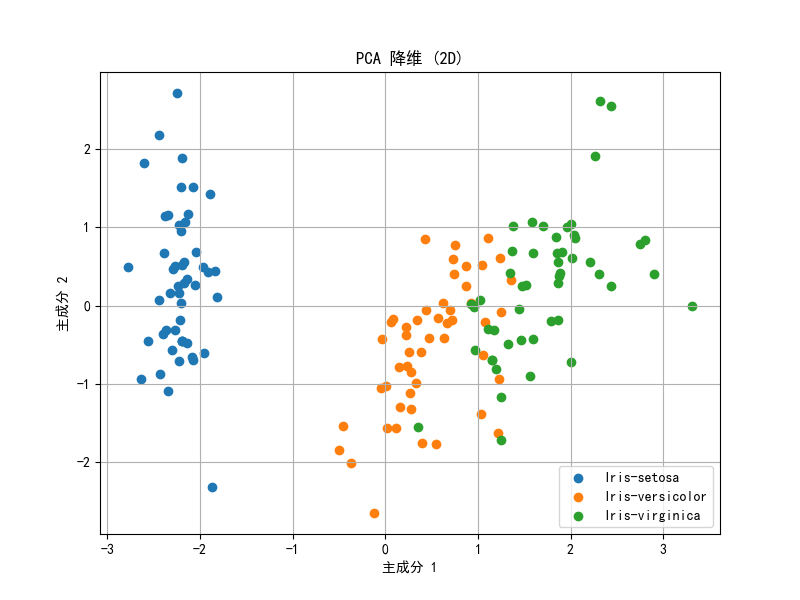
\includegraphics[width=0.8\textwidth]{2.png}
\caption{PCA 降维 (2D)}
\label{fig:pca_2d}
\end{figure}

\begin{figure}[H]
\centering
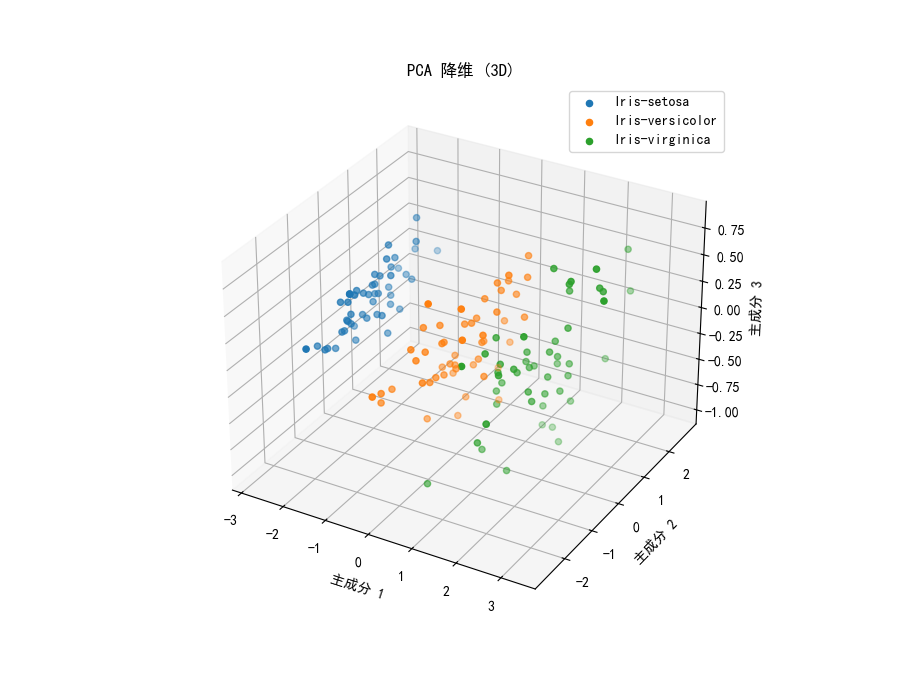
\includegraphics[width=0.8\textwidth]{3.png}
\caption{PCA 降维 (3D)}
\label{fig:pca_3d}
\end{figure}

\section{实验总结}
我通过实验掌握了 K-Means 聚类和 PCA 降维算法的实现方法，并通过实验验证了它们在实际应用中的有效性。同时，我还学习了如何使用可视化手段分析数据的内在结构。

\newpage
\appendix
\section{完整代码}

\begin{lstlisting}[language=Python]
import numpy as np
import matplotlib.pyplot as plt
from sklearn.cluster import KMeans
from sklearn.metrics import accuracy_score, silhouette_score
from sklearn.decomposition import PCA
from sklearn.preprocessing import StandardScaler
from mpl_toolkits.mplot3d import Axes3D
from scipy.stats import mode

plt.rcParams['font.sans-serif'] = ['SimHei']
plt.rcParams['axes.unicode_minus'] = False

data = np.loadtxt('iris.data', delimiter=',', dtype=str, usecols=range(5))
X = data[:, :4].astype(float)
target_names_str = data[:, 4]
unique_labels = np.unique(target_names_str)
y = np.array([np.where(unique_labels == label)[0][0] for label in target_names_str])
target_names = unique_labels

X_kmeans = X[:, 2:4]
scaler = StandardScaler()
X_kmeans = scaler.fit_transform(X_kmeans)
kmeans = KMeans(n_clusters=3, max_iter=100, random_state=42)
y_pred = kmeans.fit_predict(X_kmeans)
labels = np.zeros_like(y_pred)
for i in range(3):
    mask = (y_pred == i)
    labels[mask] = mode(y[mask], keepdims=True)[0]
acc = accuracy_score(y, labels)
print("K-Means 聚类准确率：", acc)
sil_score = silhouette_score(X_kmeans, y_pred)
print("K-Means 轮廓系数：", sil_score)

plt.figure(figsize=(8, 6))
for i in range(3):
    plt.scatter(
        X_kmeans[y_pred == i, 0],
        X_kmeans[y_pred == i, 1],
        label=f'聚类 {i}'
    )
plt.scatter(
    kmeans.cluster_centers_[:, 0],
    kmeans.cluster_centers_[:, 1],
    c='red',
    marker='X',
    s=200,
    label='中心点'
)
plt.title("K-Means 聚类结果 (Iris)")
plt.xlabel("特征 3")
plt.ylabel("特征 4")
plt.legend()
plt.grid()
plt.show()


X_scaled = scaler.fit_transform(X)
pca_2d = PCA(n_components=2)
X_pca_2d = pca_2d.fit_transform(X_scaled)
print("PCA (2D) 方差贡献率：", pca_2d.explained_variance_ratio_)
print("累计方差贡献率：", np.sum(pca_2d.explained_variance_ratio_))

plt.figure(figsize=(8, 6))
for i in range(3):
    plt.scatter(
        X_pca_2d[y == i, 0],
        X_pca_2d[y == i, 1],
        label=target_names[i]
    )
plt.title("PCA 降维 (2D)")
plt.xlabel("主成分 1")
plt.ylabel("主成分 2")
plt.legend()
plt.grid()
plt.show()

pca_3d = PCA(n_components=3)
X_pca_3d = pca_3d.fit_transform(X_scaled)
print("PCA (3D) 方差贡献率：", pca_3d.explained_variance_ratio_)
print("累计方差贡献率：", np.sum(pca_3d.explained_variance_ratio_))

fig = plt.figure(figsize=(9, 7))
ax = fig.add_subplot(111, projection='3d')
for i in range(3):
    ax.scatter(
        X_pca_3d[y == i, 0],
        X_pca_3d[y == i, 1],
        X_pca_3d[y == i, 2],
        label=target_names[i]
    )
ax.set_title("PCA 降维 (3D)")
ax.set_xlabel("主成分 1")
ax.set_ylabel("主成分 2")
ax.set_zlabel("主成分 3")
ax.legend()
plt.show()

\end{lstlisting}

\end{document}